% ===== 原文 pp.72--76 =====
% 接续：p.71 末句「在经典极限 $r\to\infty$ 下，量子的」在本块开头续完。
% 块边界：本块写到 p.76 的 (7.15) 及其后的解释句为止
%（该句跨到 p.77 开头「the length of the j-th row)…N_\ell=N.」，按「跨页句子由开始者写完」由本块写完）；
% 下一块 tr-06 自 p.77 的「味对称性为 (7.16)」起。

% [原文 p.72]
数 $w^{(k)}(\alpha)$ 简化为 $\fg$ 的 Casimir 不变量，
而 OPE (7.3) 变成 $\phi_k$ 在驯服穿刺点附近的奇点性 [19]。

量子数 $w^{(k)}(\alpha)$ 在 Weyl 群作用 $\alpha\mapsto Q+w(\alpha-Q)$ 下不变，
其中 $w:\fh^*\to\fh^*$ 是任意 Weyl 群元素。
因此 $V_\alpha$ 与 $V_{Q+w(\alpha-Q)}$ 有相同的量子数；
在 Toda 共形场论中它们是同一个算子，至多相差一个称为反射振幅的归一化，
后者在 [333--335] 中确定。对一般的 $\alpha$，这些表达式可以改写成如下陈述 [93]
\footnote{[333--335] 中与同一批作者后来的工作 [136] 中的反射振幅似乎相差一个符号。
我取后者的符号为正确，因为它似乎与 Liouville 共形场论相符。}
\begin{equation}
\widehat{V}_\alpha
=\frac{\lambda^{\langle\rho,\alpha-Q\rangle}}
{\prod_{e>0}\Upsilon_b\big(\langle Q-\alpha,e\rangle\big)}\,V_\alpha(z)
\tag{7.4}
\end{equation}
在 $\alpha$ 的 Weyl 反射下不变，其中乘积遍历全部正根 $e$，
并回忆 $\lambda=[\pi\Gamma(b^2)\mu/\Gamma(1-b^2)]^{1/b}$。
虽然常常方便，但归一化 (7.4) 在分母发散的 $\alpha$ 取值处并无意义。

Toda 共形场论的算子谱由顶点算子 $V_{Q+a}$ 组成，其中 $a\in\fh$（按我们的约定为纯虚），
并对 Weyl 群取模。其中每一个都是 $W_\fg$ 代数一个 Verma 模的最高权态，没有零态。
与 Virasoro 代数的情形一样，也存在某些动量值（离这条线）使顶点算子带零后代。
确切的条件
\footnote{这一点是用屏蔽荷得到的，例如见 [336]。
读现代文献时我觉得零后代应从能级 $n_1n_2$ 开始，但我在旧的 Toda 共形场论文献中没找到合适的出处。欢迎指正。}
是：若对某个根 $e$ 与正整数 $n_1,n_2>0$ 有 $\langle\alpha-Q,e\rangle=-n_1b-n_2/b$，
则 $V_\alpha$ 带零后代。

\para{Toda 共形场论中的关联函数。}
$W_\fg$ 对称性严重限制 Toda 共形场论中的两点与三点函数。
主算子 $V_{\alpha_1}$ 与 $V_{\alpha_2}$ 的两点函数只有在它们的量子数满足
$w^{(k)}(\alpha_1)=(-1)^kw^{(k)}(\alpha_2)$ 时才非零，
因此（在 Weyl 群作用下）$\alpha_1=2Q-\alpha_2$。
考虑到我们偏好的归一化 (7.4)，有
\begin{equation}
\langle\widehat{V}_\alpha(z,\bar z)\widehat{V}_{\alpha'}(0)\rangle
=|z|^{-4h(\alpha)}
\frac{\sum_{w\in\mathrm{Weyl}}\delta_{Q-\alpha'=w(\alpha-Q)}}
{\prod_{\text{roots }e}\Upsilon_b\big(\langle Q-\alpha,e\rangle\big)},
\tag{7.5}
\end{equation}
其中 delta 函数之和只是用来保证 Weyl 不变性；
而若改用未归一化的 $V_\alpha$（这在处理部分退化动量时是必需的），
这个和里会相应出现一些反射振幅。
$W_\fg$ 后代的两点函数构成的 Shapovalov 矩阵按标准方式、通过交换 W 代数模 $W^{(k)}_n$ 得到。
我们的归一化选择之所以讨人喜欢，是因为如同 $\fsu(2)$ 情形，
逆两点函数 $\prod_e\Upsilon_b(\langle Q-\alpha,e\rangle)$
恰好与规范代数 $\fg$ 的矢量多重态的单圈行列式相符。

主算子的三点函数编码在系数 $\widehat{C}_{123}=\widehat{C}(\alpha_1,\alpha_2,\alpha_3)$ 中
\begin{equation}
\langle\widehat{V}_{\alpha_1}(z_1,\bar z_1)\widehat{V}_{\alpha_2}(z_2,\bar z_2)
\widehat{V}_{\alpha_3}(z_3,\bar z_3)\rangle
=\frac{\widehat{C}(\alpha_1,\alpha_2,\alpha_3)}
{|z_1-z_2|^{2h_{12}}|z_1-z_3|^{2h_{13}}|z_2-z_3|^{2h_{23}}},
\tag{7.6}
\end{equation}

% [原文 p.73]
其中 $h_{ij}=h(\alpha_i)+h(\alpha_j)-h(\alpha_k)$。
一般的三点函数并不知道；此外，与 Virasoro 后代的通常情形不同，
大多数 $W_\fg$ 后代的三点函数无法用 $\widehat{C}_{123}$ 表达。
只有下文讨论的某些特殊情形 [136, 337, 338] 已被确定。

\para{欠定的共形块。}
这对 Toda 共形场论的高点关联函数有连锁影响：
描述 $W_\fg$ 后代如何贡献的共形块并不被对称性固定。例如考虑
\begin{equation}
\langle\widehat{V}_{\alpha_1}\widehat{V}_{\alpha_2}\widehat{V}_{\alpha_3}
\widehat{V}_{\alpha_4}\rangle
=\int_{a\in\fh/\mathrm{Weyl}}\dd a\;\sum_{Y}
\langle\widehat{V}_{\alpha_1}\widehat{V}_{\alpha_2}\widehat{V}^{[Y]}_{Q-a}\rangle\,
\frac{1}{\langle\widehat{V}_{Q-a}\widehat{V}_{Q+a}\rangle}\,
\langle\widehat{V}^{[Y]}_{Q+a}\widehat{V}_{\alpha_3}\widehat{V}_{\alpha_4}\rangle,
\tag{7.7}
\end{equation}
其中我们略去了空间依赖性，积分遍历谱中的主算子 $\widehat{V}_\alpha$，
求和遍历它们的后代（已正交化，并归一化到与主算子有相同的模 $\langle\widehat{V}_{Q-a}\widehat{V}_{Q+a}\rangle$）。
对一般的 $\alpha_i$，由主三点函数所决定的三点函数 $\langle\widehat{V}_{\alpha_1}\widehat{V}_{\alpha_2}\widehat{V}^{[Y]}_{Q-a}\rangle$，
只有那些 $\widehat{V}^{[Y]}_{Q-a}$ 实际上是 $\widehat{V}_{Q-a}$ 的 Virasoro 后代的情形。
由带三个满驯服穿刺点的三穿刺球面得到的 class S 理论是非拉氏量的 tinkertoy $T_\fg$，
超对称局域化对其球面配分函数无话可说。
一条非常有力的迂回途径是考虑 5d 提升，
并求出 $S^4_b\times S^1$ 配分函数在圆周半径 $\beta$ 收缩时的极限 [339--342]。
原则上这给出 $\widehat{C}_{123}$ 与全部后代三点函数的猜想表达式 [343]，
但不确定 $\beta\to 0$ 极限是否存在，
也不清楚如何把拓扑顶点形式的参数与后代的基底联系起来，详见 [229]。
高点关联函数对应于把若干份 $T_\fg$ 规范耦合在一起所得的理论。
由于规范群每根管子只有一个因子 $G$，瞬子模空间是已知的，
瞬子配分函数就是该空间上的某个积分。
然而被积函数依赖于物质理论 $T_\fg$，而后者对瞬子的反应并不知道。
这与下述情形完全类似：后代的求和已知，但所需的三点函数并不能由 $\widehat{C}_{123}$ 导出。

% [Tutor Note: p.73 式 (7.7) 与 p.64 式 (6.7) 的对照要点：Virasoro 情形下后代的归一化只需 $g^{-1}_{56}$，
%   因为后代数目由 Verma 模的能级给出且三点函数全由 $C_{ijk}$ 决定；而 $W_\fg$ 有 $\rank\fg$ 个生成元，
%   后代空间更大，$\widehat C_{123}$ 不足以决定 $\langle\widehat V_{\alpha_1}\widehat V_{\alpha_2}\widehat V^{[Y]}_{Q-a}\rangle$。
%   这也正是「半退化」动量重要性的来源：有 level-1 零矢量后，$W_N$ 生成元可化到 Virasoro 生成元。
%   核对锚点：$\fg=\fsu(2)$ 时 $\rank\fg=1$、$W_{\fsu(2)}=\mathrm{Vir}$，(7.7) 应退化为 (6.6)--(6.7) 的形式。]

\subsection{高阶 AGT 对应}

class S 理论的主要构件是联系着三个满驯服穿刺点的 tinkertoy $T_\fg$，综述见 [117]。
当 $\fg\ne\fsu(2)$ 时，这一 tinkertoy 是非拉氏量的
\footnote{有趣的是，它的 3d $\cN=4$ 维数约化在镜像对偶下给出一个由星形箭图 [344] 描述的拉氏量理论。}。
因此，高阶 AGT 对应最简单的例子------例如 $\mathrm{SU}(N)$ SQCD 配分函数与 $\fsu(N)$ Toda
共形场论四点函数的匹配------需要另一类驯服穿刺点（称为单驯服穿刺点）。

除满与单驯服穿刺点之外，还有其它驯服穿刺点（当然还有一大批野生穿刺点），
它们在 [1, 6, 261, 318, 336, 345, 346] 中被研究。
Chacaltana 与 Distler 及其合作者在 [95, 97, 100--106, 108] 中开展了对 tinkertoy 分类的大型研究计划
（不过要提醒一句：他们在这一语境中对「非正则（irregular）」一词的用法并不标准）。
在黎曼面中某根管子被捏紧的极限下可能出现的穿刺点，在 [8, 347] 中被研究。

% [原文 p.74]
各种驯服穿刺点对应于部分退化的 Toda 共形场论顶点算子 $V_\alpha$，我们以 $\fg=\fsu(N)$ 作说明。
我们还要描述如何通过调节参数把穿刺点「部分关闭」，这在规范理论一侧对应于部分 Higgs 化。
最后，我们概述如何纳入非单链的规范群。

\para{Wyllard 关系：$\mathrm{SU}(N)$ 线性箭图与一个 $\fsu(N)$ Toda 共形场论关联函数。}
为简单起见，我们此后集中在 $\fg=\fsu(N)$ 情形，它被理解得最清楚。
该手征代数有不同的记法：$W_{\fsu(N)}=W_{A_{N-1}}=W_N$。

在 4.4 小节中我们考虑过一个线性箭图规范理论，
其超多重态在 $n-1$ 个相继的 $\mathrm{SU}(N)$ 群的双基本表示中变换，其中中间 $n-3$ 个被规范化。
除箭图两端的两个 $\mathrm{SU}(N)$ 味对称性之外，$n-2$ 个超多重态中每一个都带一个 $\mathrm{U}(1)$ 味对称性。
如 (4.26) 所述，该理论通过在带 $n$ 个穿刺点的球面上约化 $\cX(\fsu(N))$ 实现，
这些穿刺点与这 $n$ 个味对称性因子相对应。
$\mathrm{SU}(N)$ 味对称性对应于满驯服穿刺点，
在那里每个微分 $\phi_k$ 在无质量情形下有一个 $k-1$ 阶极点，在打开 $\mathrm{SU}(N)$ 质量时则有一个 $k$ 阶极点。
$\mathrm{U}(1)$ 味对称性对应于单驯服穿刺点，
在无质量情形下每个 $\phi_k$ 在那里有一个一阶极点（有质量的情形更复杂）。

[93] 中提出的 AGT 对应取如下形式
\begin{equation}
Z_{S^4_b}\!\left(
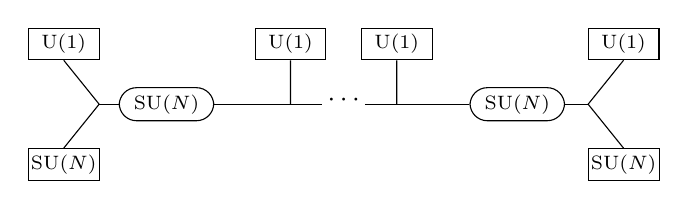
\begin{tikzpicture}[baseline=(current bounding box.center),scale=0.9,
  qnd/.style={draw,rounded corners=2.2mm,minimum height=4.2mm,minimum width=12mm,inner sep=1pt,font=\scriptsize},
  qbx/.style={draw,minimum height=4.0mm,minimum width=9mm,inner sep=1pt,font=\scriptsize}]
\node[qnd] (n1) at (0,0) {$\mathrm{SU}(N)$};
\node[qbx] (u1) at (-1.45,0.85) {$\mathrm{U}(1)$};
\node[qbx] (s1) at (-1.45,-0.85) {$\mathrm{SU}(N)$};
\coordinate (f1) at (-0.95,0);
\draw (n1.west) -- (f1);
\draw (f1) -- (u1.south);
\draw (f1) -- (s1.north);
\node[qnd] (n2) at (4.95,0) {$\mathrm{SU}(N)$};
\draw (n1.east) -- (2.2,0);
\draw (2.8,0) -- (n2.west);
\node at (2.5,0.05) {$\cdots$};
\node[qbx] (u2) at (1.75,0.85) {$\mathrm{U}(1)$};
\draw (u2.south) -- (1.75,0);
\node[qbx] (u3) at (3.25,0.85) {$\mathrm{U}(1)$};
\draw (u3.south) -- (3.25,0);
\node[qbx] (u4) at (6.45,0.85) {$\mathrm{U}(1)$};
\node[qbx] (s2) at (6.45,-0.85) {$\mathrm{SU}(N)$};
\coordinate (f2) at (5.95,0);
\draw (n2.east) -- (f2);
\draw (f2) -- (u4.south);
\draw (f2) -- (s2.north);
\end{tikzpicture}
\right)
=\big\langle\widehat{V}_{\alpha_1}\widehat{V}_{\mu_2}\widehat{V}_{\mu_3}\cdots
\widehat{V}_{\mu_{n-1}}\widehat{V}_{\alpha_n}\big\rangle^{\mathrm{Toda}(\fsu(N))}
\tag{7.8}
\end{equation}
其中 $\alpha_j$（$j=1,n$）编码两个满穿刺点的虚 $\mathrm{SU}(N)$ 质量参数，
$m_j=(m_{j1},\dots,m_{jN})$ 且 $\sum_p m_{jp}=0$；
而 $\mu_j$（$j=2,\dots,n-1$）以下述方式编码第 $j$ 个 $\mathrm{U}(1)$ 质量参数 $m_j\in i\R$：
\begin{equation}
\begin{aligned}
\alpha_j&=Q+rm_j, && j&=1,n,\\
\mu_j&=\Big(\frac{N}{2}\big(b+\frac{1}{b}\big)+rm_j\Big)\varpi_1, && j&=2,\cdots n-1.
\end{aligned}
\tag{7.9}
\end{equation}
例如在 $n=4$ 的情形，这把一个 Toda 共形场论四点函数认同为带 $N_f=2N$ 个味的 $\mathrm{SU}(N)$ SQCD 的配分函数。

% [Tutor Note: p.74 式 (7.9) 的因子数目可自检：$n$ 个味对称性因子 = 2 个 $\mathrm{SU}(N)$（满穿刺，$\alpha_1,\alpha_n$）
%   + $(n-2)$ 个 $\mathrm{U}(1)$（简单穿刺，$\mu_2,\dots,\mu_{n-1}$），与 (7.8) 右端 $n$ 个顶点算子、(7.10) 分子中
%   $n-2$ 个三点函数因子逐一对应；若 $n=4$ 则只剩 $\mu_2,\mu_3$ 两个简单穿刺，正是 Wyllard 的 $\mathrm{SU}(N)$、$N_f=2N$ 情形。
%   另注意 (7.9) 中 $\mu_j$ 只沿 $\varpi_1$ 方向（半退化），而 $\alpha_j$ 是任意的（满穿刺），这正对应本节开头
%   「一个简单穿刺 ↔ 一个半退化顶点算子」的字典。]

为理解这些动量，我们讨论相应的顶点算子 $V_\alpha$ 及其 $W_N$ 后代。
我们已经遇到过 $Q+\fh$ 中的动量，它们描述 Toda 共形场论谱中出现的可归一化态。
与第一个权 $\varpi_1$ 成正比的动量称为半退化动量：
自 [348, 349] 起人们发现，它们在能级 1 处带零的 $W_N$ 后代。
考虑一个带半退化顶点算子的三点函数 $\langle V_\alpha V_{\kappa\varpi_1}V_{\alpha'}\rangle$。
由于零矢量的存在，任意 $W_N$ 生成元的作用

% [原文 p.75]
都可以转成 Virasoro 生成元的作用，从而化作作用在已知坐标依赖性上的微分算子。
这意味着 $V_\alpha$、$V_{\kappa\varpi_1}$ 与 $V_{\alpha'}$ 的后代的三点函数，
被唯一地固定为主算子三点函数的某个倍数。

\para{检验 Wyllard 关系。}
与 $\fsu(2)$ 情形一样，匹配 (7.8) 最直接是在与球面关联函数的 s-通道分解相对应的 S 对偶框架中检验。
每个三穿刺球面片段有一个单驯服穿刺点与两个满穿刺点
（在规范理论一侧对应于一个双基本表示超多重态）。
在这个通道中展开关联函数，用主算子改写后代的三点函数，
并把后代的贡献收集进一个共形块，我们得到
\begin{equation}
\begin{aligned}
&\langle\widehat{V}_{\alpha_1}\widehat{V}_{\mu_2}\cdots\widehat{V}_{\mu_{n-1}}
\widehat{V}_{\alpha_n}\rangle\\
&\quad=\int_{\substack{a_j\in\fh/\mathrm{Weyl}\\ 2\le j\le n-2}}\dd a\;
\frac{\langle\widehat{V}_{\alpha_1}\widehat{V}_{\mu_2}\widehat{V}_{Q+a_2}\rangle
\langle\widehat{V}_{Q-a_2}\widehat{V}_{\mu_3}\widehat{V}_{Q+a_3}\rangle\cdots
\langle\widehat{V}_{Q-a_{n-2}}\widehat{V}_{\mu_{n-1}}\widehat{V}_{\alpha_n}\rangle}
{\langle\widehat{V}_{Q+a_2}\widehat{V}_{Q-a_2}\rangle\cdots
\langle\widehat{V}_{Q+a_{n-2}}\widehat{V}_{Q-a_{n-2}}\rangle}\,
\mathcal{F}(z)\overline{\mathcal{F}(\bar z)},
\end{aligned}
\tag{7.10}
\end{equation}
其中 $\mathcal{F}(z)$ 是某个共形块，它们（原则上）可以按 $C$ 的复结构参数的幂次展开计算，
并依赖于全部外部与内部动量。
共形块（对这些动量）可计算这一事实本身，
与 4d 理论是拉氏量的、因而其配分函数可用超对称局域化计算这一事实，配合得很好。

匹配的一个关键部分是：(7.10) 中的 $n-2$ 个三点函数应当与箭图中
$n-2$ 个双基本表示超多重态的单圈行列式相符。
所幸，两个非退化与一个半退化顶点算子的三点函数 $\langle V_{\alpha_1}V_{\kappa\varpi_1}V_\alpha\rangle$
已在 [136, 337, 338] 中算出：办法是把一个完全退化的顶点算子 $V_{-b\varpi_1}$ 插入关联函数，
并求解由此得到的微分方程。
\footnote{这一自举技巧是 Teschner 为求解 Liouville 共形场论而引入的。
在 Toda 共形场论语境下对更一般的完全退化顶点算子的进一步探索，
另见 [68, 350--352]；其它相关关联函数见 [353, 354]。}
考虑非退化算子的归一化 (7.4)，再取一个权宜的归一化
\begin{equation}
\widehat{V}_{\kappa\varpi_1}
=\frac{\lambda^{\langle\kappa\varpi_1,\rho\rangle}}
{\big(\Upsilon_b(b)\big)^{N-1}\Upsilon_b(\kappa)}\,V_{\kappa\varpi_1}
\tag{7.11}
\end{equation}
它虽在 Weyl 变换下不变，却是对记号的一种滥用，
因为这里的 $\widehat{V}$ 与 $V$ 的关系并不像 (7.4) 那样。
于是三点函数为 [136]
\begin{equation}
\widehat{C}(Q+a_1,\kappa\varpi_1,Q+a_2)
=\frac{1}{\prod_{i,j=1}^{N}\Upsilon_b\big(\kappa/N-\langle a_1,h_i\rangle-\langle a_2,h_j\rangle\big)}
\tag{7.12}
\end{equation}
其中 $h_i$ 是 $\fsu(N)$ 基本表示的权。
这些 Upsilon 函数的乘积确实与 $N^2$ 个超多重态的单圈行列式相符，

% [Tutor Note: p.75 式 (7.12) 的两个自检点：(i) 乘积共 $N^2$ 个因子，与正文所说
%   「$N^2$ 个超多重态的单圈行列式」一致；(ii) (7.11) 的分母 $(Υ_b(b))^{N-1}$ 的幂次 $N-1$ 正是 $\fsu(N)$
%   简单根的个数（也是 $\varpi_1$ 的 Dynkin 标号），可用来核对是否抄错了指数。
%   另：$\kappa/N$ 的归一化使 $\kappa$ 与第 $j$ 个 $\mathrm{U}(1)$ 质量 $m_j$ 通过 $\mu_j$ 的 $\varpi_1$ 系数相联系，
%   代入 $a_1=a_2=0$ 时 $\widehat C\to\prod_{i,j}Υ_b(\kappa/N)^{-1}=Υ_b(\kappa/N)^{-N^2}$。]

% [原文 p.76]
即 $S^4_b$ 上、带适当质量的 $N^2$ 个超多重态的单圈行列式。
逆两点函数则与矢量多重态的单圈行列式相符，见 (7.5) 之后。
经典作用量也正确地重现了 Toda 共形场论关联函数的领头 $z$ 依赖性。
最后，还可以不厌其烦地逐阶把共形块与瞬子配分函数匹配起来，以确认 (7.8)。

(7.8) 中的 Toda 关联函数原则上可以在许多其它通道中分解。
例如在四点函数（$n=4$）中取半退化顶点算子 $\widehat{V}_{\mu_1}$ 与 $\widehat{V}_{\mu_2}$ 的 OPE，
就得到 t-通道分解。在 $N=3$ 情形，这一融合产生的内部动量是非退化的，
因此该分解涉及一般的三点函数。
$\mathrm{SU}(3)$ SQCD 相应的 S 对偶框架由 $T_{\fsu(3)}$ tinkertoy（即 $e_6$ Minahan--Nemeschansky SCFT）
与一些超多重态经某个规范群耦合而成，该规范群结果是 $\mathrm{SU}(2)$。
对一般的 $N$，这类融合导致介于满穿刺点与单驯服穿刺点之间的大量穿刺点类型。

\para{部分 Higgs 化。}
考虑 (7.8) 中的线性箭图。其 Higgs 分支由超多重态标量获得 VEV 的超对称真空组成。
走到 Higgs 分支上任一给定点后，超多重态的 VEV 可能把规范对称性破缺到更小的群，
从而把箭图缩减为更小的箭图。

我们把双基本表示超多重态中的标量记作 $(Q_j,\widetilde{Q}_j)$，$j=2,\dots,n-1$。
一类重要的真空来自给最左边 $\mathrm{SU}(N)$ 味对称性群的矩映射施加幂零 VEV
（例如见 [355] 的附录）
\begin{equation}
\mu_1=\widetilde{Q}_2Q_2-\frac{1}{N}\Tr(\widetilde{Q}_2Q_2)
\tag{7.13}
\end{equation}
$\fsu(N)_\C=\mathfrak{sl}(N,\C)$ 中的幂零矩阵在共轭意义下由 $N$ 的一个分拆分类，
等价地由一个含 $N$ 个方块的杨图 $Y$ 分类。
记 $n_k$ 为 $Y$ 中长度为 $k$ 的列数，则我们考虑的幂零 VEV 取块对角形式
\begin{equation}
\langle\mu_1\rangle
=J_1^{\oplus n_1}\oplus J_2^{\oplus n_2}\oplus\cdots\oplus J_\ell^{\oplus n_\ell}
\tag{7.14}
\end{equation}
其中 $J_k$ 是 $k\times k$ 的 Jordan 块，共 $n_k$ 个（例如 $J_1=(0)$）。
VEV $\langle\mu_1\rangle$ 不能孤立地施加，
因为 F-项关系会使得超多重态 $(Q_j,\widetilde{Q}_j)$（$j=2,\cdots,\ell$）取到非零值。

Higgs 机制于是破缺多个规范对称性。
具体地说，它把箭图最前面几个群缩减为一个\emph{箭图尾巴}
\begin{equation}
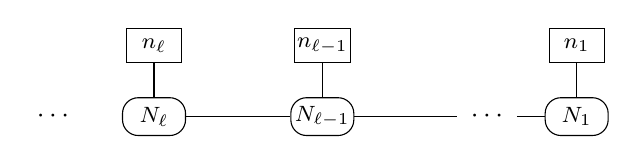
\begin{tikzpicture}[baseline=(current bounding box.center),scale=0.95,
  tnd/.style={draw,rounded corners=2.0mm,minimum height=4.8mm,minimum width=8mm,inner sep=1pt,font=\footnotesize},
  tbx/.style={draw,minimum height=4.4mm,minimum width=7mm,inner sep=1pt,font=\footnotesize}]
\node at (-1.25,0) {$\cdots$};
\node[tnd] (na) at (0.1,0) {$N_\ell$};
\node[tbx] (ba) at (0.1,0.95) {$n_\ell$};
\draw (ba.south) -- (na.north);
\node[tnd] (nb) at (2.35,0) {$N_{\ell-1}$};
\node[tbx] (bb) at (2.35,0.95) {$n_{\ell-1}$};
\draw (bb.south) -- (nb.north);
\draw (na.east) -- (nb.west);
\node[tnd] (nc) at (5.75,0) {$N_1$};
\node[tbx] (bc) at (5.75,0.95) {$n_1$};
\draw (bc.south) -- (nc.north);
\draw (nb.east) -- (4.15,0);
\node at (4.55,0) {$\cdots$};
\draw (4.95,0) -- (nc.west);
\end{tikzpicture}
\tag{7.15}
\end{equation}
其中圆节点是 $\mathrm{SU}(N_j)$ 规范群，矩形计数基本表示超多重态，
而 $N_j$ 由 $N_0=0$ 与 $N_j-N_{j-1}=n_j+n_{j+1}+\cdots+n_\ell$ 确定（后者即第 $j$ 行的长度）。
换言之，$N_j$ 计数第 $1,\cdots,j$ 行中的全部方块，特别地 $N_\ell=N$。

% [Tutor Note: p.76 式 (7.15) 后的公式可用杨图直接核验：设 $n_k$=长度为 $k$ 的列数，
%   则第 $1..j$ 行的方块数 $N_j=\sum_k n_k\min(j,k)$，于是
%   $N_j-N_{j-1}=\sum_{k\ge j}n_k=n_j+n_{j+1}+\cdots+n_\ell$，与原文一致；
%   又 $N_\ell=\sum_k k\,n_k=N$（$Y$ 恰有 $N$ 个方块），与「特别地 $N_\ell=N$」自洽。
%   另核 (7.14)：$\sum_k k n_k=N$ 也保证 $\langle\mu_1\rangle$ 是 $\fsu(N)$ 中的幂零元（$J_k$ 为 $k\times k$ 块）。]

% [Tutor Note: p.70 的灰底要点框在原文中并无标题条（§1--§6 各节的要点框都带粗体标题条），
%   故 p.70 处 keybox 的标题参数留空，以忠实反映原文版式；若编译后出现一条空白深色标题条，
%   那是排版副作用，可在 preamble 的 keybox 定义中加 no-title 处理。]
